
\documentclass[14pt,aspectratio=1610]{beamer} %,draft  % !TEX program = xelatex


% \usefonttheme{sanserif}

% \usetheme{Pittsburgh}%
\usecolortheme{orchid}


\setbeamersize{text margin left=.25in,text margin right=.25in}
\setbeamersize{sidebar width left=1cm, sidebar width right=1cm}

\setbeamertemplate{sidebar right}{}
\setbeamertemplate{footline}{%
\hfill
\hspace{1cm}\insertframenumber{}} %/\inserttotalframenumber

\usepackage{graphicx}
\graphicspath{{./diagrams/}}
% \graphicspath{{diagrams/}}

\usepackage{amssymb, amsfonts, amsmath}
\usepackage[outdir=./diagrams/]{epstopdf}



\newcommand{\C}{\mathbb{C}}
\newcommand{\bR}{\mathbb{R}}
\newcommand{\bP}{\mathbb{P}}

\newcommand{\sE}{\mathcal{E}}
\newcommand{\sL}{\mathcal{L}}
\newcommand{\sM}{\mathcal{M}}
\newcommand{\sS}{\mathcal{S}}


\newcommand{\vpad}[1]{\raise0.5pt\hbox{\vphantom{$#1$}}#1}
% \newcommand{\vpad}[1]{#1}
\newcommand{\overbar}[1]{\mkern1.5mu\overline{\mkern-1.5mu#1\mkern-1.5mu}\mkern1.5mu}
% \newcommand{\overbar}[1]{#1}

\newcommand{\Tb}{\overbar{\vpad\Theta}}
\newcommand{\boldG}{\mathbf{G}}
\newcommand{\Gb}{\overbar{\vpad\boldG}}
\newcommand{\CL}{\mathcal{L}}
\newcommand{\Lb}{\overbar{\vpad\LL}}
\newcommand{\Z}{\mathbf{Z}}
\newcommand{\Zb}{\overbar{\vpad\Z}}
\newcommand{\D}{\mathbf{D}}
\newcommand{\Db}{\overbar{\vpad\D}}
\newcommand{\zz}{\mathbf{z}}
\newcommand{\zzb}{\overline\zz}


\newcommand{\bF}{\mathbf{f}}
\newcommand{\bx}{\mathbf{x}}
\newcommand{\bp}{\mathbf{p}}

\newcommand{\calC}{\mathcal{C}}
\newcommand{\calK}{\mathcal{K}}

\newcommand{\jth}{$j^{\textnormal{th}}$}

\newcommand{\x}{\mathbf{x}}
\newcommand{\z}{\mathbf{z}}
\newcommand{\y}{\mathbf{y}}
\newcommand{\p}{\mathbf{p}}

\usepackage{multirow}
\usepackage[normalem]{ulem}


\usepackage[]{listings}
\lstset{
language=C++,
               basicstyle=\ttfamily,
                keywordstyle=\color{blue}\ttfamily,
                stringstyle=\color{red}\ttfamily,
                commentstyle=\color{green}\ttfamily,
                morecomment=[l][\color{magenta}]{\#}}


\usepackage{coloremoji}
\setbeamertemplate{footline}[frame number] % except I kind of like 
                                           % including the frame number
\title[Git @ ICERM \hspace{2.5in} Brake]{A \LaTeX-oriented intro to Git \\  \small the tex part is in the interactive demo not in the slides}
\author{Danielle Amethyst Brake}
\date{22 October, 2018}




\newcommand{\fframe}[2]{
   \begin{frame}
\frametitle{#1}
#2
\end{frame}
}

\newtheorem{concl}{Conclusion}

\usepackage{verbatim}

\usepackage{hyperref}

\begin{document}
\setbeamertemplate{navigation symbols}{}


%----------- titlepage ----------------------------------------------%
\begin{frame}

 \titlepage
 
 \begin{center}
 ICERM Semester on Nonlinear Algebra \\ Inter-week collaboration time
\end{center}

  \includegraphics[height=0.5in]{UWEC-stacked-wordmark-Blue_cmyk}
\hfill
 \includegraphics[height=0.5in]{Power-of-AND_stckd_blu_CMYK}

\end{frame}


\AtBeginSection[]
{

{
\usebackgroundtemplate{
\includegraphics[width=\paperwidth]{diagrams/crystalbackground.jpg}}%


  \begin{frame}
      \frametitle{Outline}
      \tableofcontents[currentsection]
  \end{frame}
  }
}













%                              _________ _       _________ _______  _______ 
%                              \__   __/( (    /|\__   __/(  ____ )(  ___  )
%                                 ) (   |  \  ( |   ) (   | (    )|| (   ) |
%                                 | |   |   \ | |   | |   | (____)|| |   | |
%                                 | |   | (\ \) |   | |   |     __)| |   | |
%                                 | |   | | \   |   | |   | (\ (   | |   | |
%                              ___) (___| )  \  |   | |   | ) \ \__| (___) |
%                              \_______/|/    )_)   )_(   |/   \__/(_______)
                                             

\section{Day 1 -- Intro to git}

\fframe{}
{
	\begin{center}

\includegraphics[height=3.5in]{diagrams/git_2x.png}\\xkcd 1597
	\end{center}
}

\fframe{What is git?}
{
\begin{definition}
	{\tt git} is a command-line program that records differences in files.
\end{definition}
\vspace{\baselineskip}

	{\em and how is that different from github?}

\vspace{\baselineskip}
	good question, my friend.  
	\begin{definition}
	GitHub is social media site build around {\tt git} repositories.  
	\end{definition}
}


\fframe{What are words related to Git?}
{
	\begin{columns}[t]
	\column{2in}
	Repo-focused words
	\begin{itemize}
		\item version control software
		\item repository / repo
		\item commit
		\item clone
		\item remote
		\item reset
		\item {\tt .gitignore}


		
	\end{itemize}

	\column{2in}
	Commit-focused words
	\begin{itemize}		
		\item branch
		\item rebase
		\item fast-forward
		\item merge
		\item fetch
		\item pull
		\item conflict
	\end{itemize}
	\end{columns}
}





\fframe{What's a commit?}{
A commit is a set of differences, additions and subtractions, together with a message describing them
}

\fframe{What's a repo?}
{  
A repository is a folder, together with a subfolder containing special git files.  Don't screw with these files.
}
                    
\fframe{What should I version control?}
{
	✅ Use git for these: 
	\begin{itemize}
		\item Files that can be meaningfully-diffed (think text files), and 
		\item static non-diffable files (think images that don't change)
	\end{itemize}

\vspace{\baselineskip}

	🚫 do NOT use git for version control for these:
	\begin{itemize}
		\item generated files (pdf's, executables)
		\item temporary files
		\item word documents (but you wouldn't use word anyway, would you? 😦)
	\end{itemize}
}






\fframe{How do i make a repository?}
{
	\begin{enumerate}
		\item make a new folder, or move to an existing one
		\item {\tt git init}
	\end{enumerate}

\vspace{\baselineskip}

👀	look around in the folder.  does it look different?
}


\fframe{How do i commit?}
{
	\begin{enumerate}
		\item make some changes
		\item {\tt git add filename.ext}
		\item {\tt git commit}
		\item write a commit message
		\item save `file' for commit message, done
	\end{enumerate}
}

\fframe{What's a good commit message?}
{
	\begin{enumerate}
		\item a short summary, like 3-10 words
		\item some longer description
	\end{enumerate}

\begin{itemize}
		\item 🚫 no vague crappy messages that utterly fail to describe your changes
		\item ✅ a message to your future self
	\end{itemize}
}

\fframe{How do I prevent myself from adding temp files?}
{
	🔴 Be very careful to not ever add a temp file, because once it starts tracking, it's there forever.  

\vspace{\baselineskip}
	Use {\tt .gitignore}, a file at root level (in the repo), that describes patterns for files to ignore.

\vfill
	protip: they're cumulative in subdirectories, and you can un-ignore things too
}


\fframe{How do I delete files?}
{
	\begin{enumerate}
		\item Delete the file in your local clone
		\item {\tt git add deletedfile.ext}
		\item {\tt git commit}
	\end{enumerate}

	or just

	\begin{enumerate}
		\item {\tt git delete file} -- all in one
	\end{enumerate}
}


\fframe{What if I mess up?}
{
	Don't mess up.   JK, but seriously, don't mess up.

\vspace{\baselineskip}

	You cannot delete commits from a repo.  
	\begin{itemize}
		\item You {\bf revert} them with the inverse commit.   
		\item You can delete branches... and maybe lose work
		\item You can delete repos... and maybe lose work
	\end{itemize}
}









\fframe{Things I haven't talked about yet}
{
	\begin{itemize}
		\item {\bf Merge conflicts} -- helping solve the ``hot copy'' problem
		\item GitHub
		\item Alternatives to GitHub
		\item Using Git as a time machine
		\item Alternatives to Git
		\item Branching models
		\item Rebasing, pulling, fast-forwarding
	\end{itemize}
}


\section{Day 2 -- GitHub}

\fframe{GitHub-specific things}
{
		\begin{columns}[t]
	\column{2in}
	Repo-focused words
	\begin{itemize}
		\item fork
		\item clone
		\item issue


		
	\end{itemize}

	\column{2in}
	Commit- or branch-focused words
	\begin{itemize}		
		\item pull request
	\end{itemize}
	\end{columns}
}




\fframe{}
{\begin{center}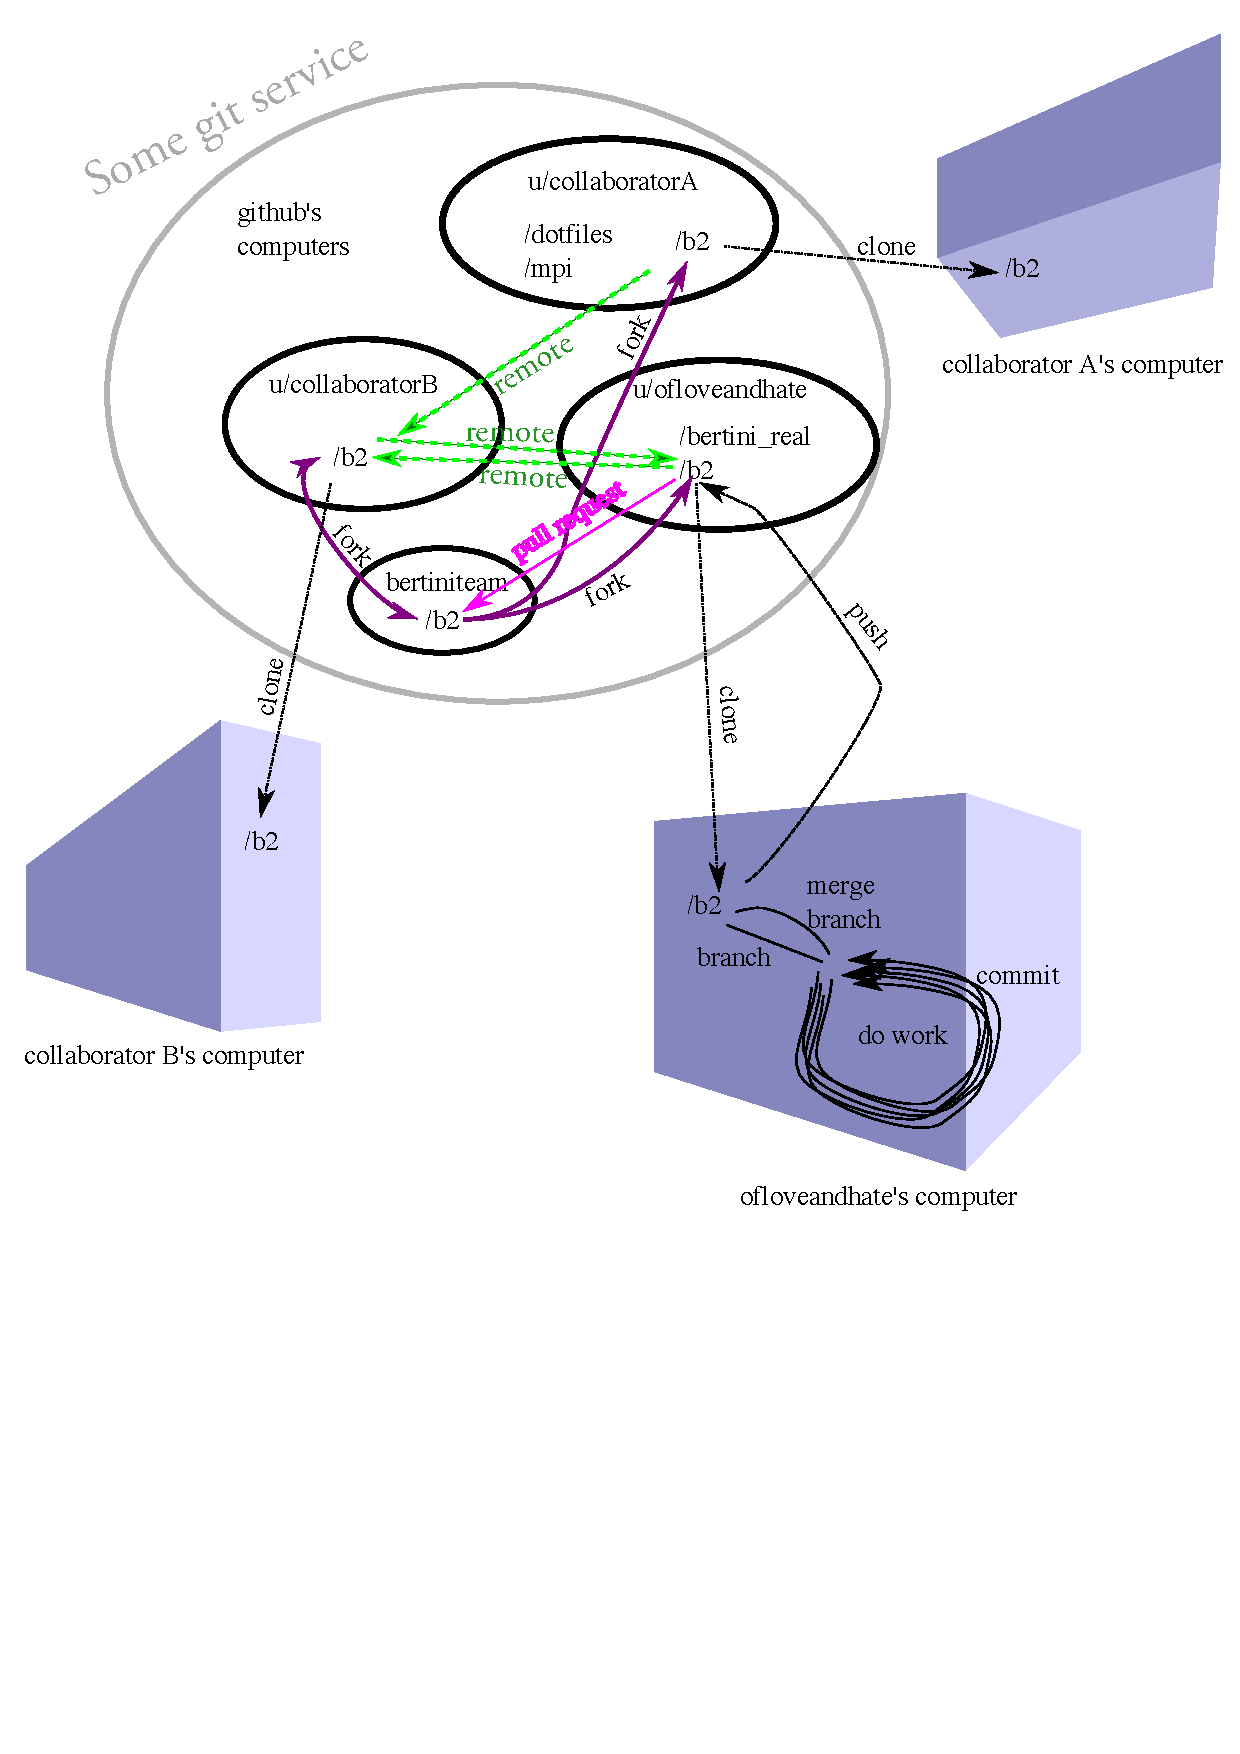
\includegraphics[width=4in]{git_usage.pdf}\end{center}}


\fframe{Game plan for teaching}
{
	\begin{enumerate}
 
		\item make a new repo on github.  clone
		\item commit
		\item push 
		\item remotes
		\item pulling and pushin
		\item merges and conflicts

	\end{enumerate}
}



\fframe{new}
{Make a git repository on Github.  If you pay, you can make them private

\vspace{\baselineskip}

\qquad $\rightarrow$ Yes, I pay for that service \\
\qquad $\Rightarrow$ (no, i don't, they have free4academic going)

\vspace{\baselineskip}

🎯 we won't make a repo on our local computer this time
}

\fframe{What is a clone?}
{
\begin{definition}
	A {\bf clone} is a repo that has been ``cloned'' from another with {\tt git clone}.  The source is a {\em remote}
\end{definition}

	\vspace{\baselineskip}

	\begin{itemize}
		\item It's a copy of the original repo, in terms of commits.  
		\item It's only an identical copy when cloned.  it's expected to diverge by committing...
	\end{itemize}
}

\fframe{clone}
{
	on your local machine, from the terminal, type

\vspace{\baselineskip}

	{\tt git clone https://github.com/username/reponame}

\vspace{\baselineskip}
and then {\tt ls} and 👀 around.  
}

\fframe{commit}
{
while 1
\begin{enumerate}
	\item make some changes
	\item {\bf add} the changed files
	\item {\bf commit}
\end{enumerate}
}



\fframe{get that data online}
{
	now we'll push.
	\begin{definition}
to {\bf push} is a git action, meaning to make a sequence of {\em commits} appear in another repo
	\end{definition}

	\vspace{\baselineskip}

	\begin{itemize}
	\item all existing commits in {\tt remote} must be present to push.  
	\item hence, pull before you push.  this often makes no difference in a one-person project
	\item typically, you push to origin, which is where the repo came from when cloned
	\end{itemize}
}





\fframe{collaborative projects using git}
{
	there are many ways to use git to share code (focusing on github here).  \\here are 2 main ways"

\vspace{\baselineskip}
	\begin{itemize}
	\item add all members as collaborators, all people commit directly to repo
	\item each person forks, and resolve via pull requests
\end{itemize}

\vspace{\baselineskip}

they both have advantages and disadvantages.  We get to choose.  
	\begin{itemize}
	\item Collaborating will lead to merge conflicts sooner
	\item Forking will let us learn about forking and PR's
\end{itemize}
}




\fframe{Fork}
{
	\begin{definition}
to {\bf fork} is a Github action, meaning to take a clone from one user's repository, and associate it as upstream
	\end{definition}

	\begin{definition}
we say A is {\bf upstream} of B when A is a remote of B, and Github has stored that direction in the association graph
	\end{definition}

	let's use that diagram again
}










\fframe{pull, fetch, merge -- defn}
{
\begin{definition}
to {\bf pull} is a git action, meaning to fetch-and-merge from a remote
	\end{definition}

	\begin{definition}
to {\bf fetch} is a git action, to query available branches and commits
	\end{definition}

\begin{definition}
to {\bf merge} is a git action, meaning to make a sequence of commits appear in the current repo.  you get the commits from a branch, either {\em locally} or from a {\em remote}
	\end{definition}

	some speech using the diagram is necessary here
}


\fframe{merge conflict}
{
	git tracks diffs on diffable files.  it's pretty smart about disjoint modifications to a file, but sometimes... it can't tell what you want to do.

		\begin{itemize}
	\item a merge conflict isn't bad
	\item the conflict is resolved when the conflicted file is marked as saved.  
	\item i honestly use a visual tool for this and don't know how to do it command line.  
	\item i totally use visual diff tools.  
\end{itemize}
}






\section{branching}

\fframe{What if I have multiple things to work on at once?}
{
	{\bf Branches} solve the problem of working on multiple facets of a project.  They're separate commit-sequences that you can make converge by {\tt merging}

	\vspace{\baselineskip}

	\begin{itemize}
		\item Make a new branch via {\tt git branch newbranchname}
		\item Convege a branch into your current by {\tt git merge branchtomerge}
		\item Get a branch from a remote via {\tt git checkout existingbranchname}
		\item Update your branch list and commit status with {\tt git fetch [remotename]}
	\end{itemize}

	We'll visit branches next time, if there is a next time
}


stuff and things i hope this generates a merge conflict



{
	
\usebackgroundtemplate{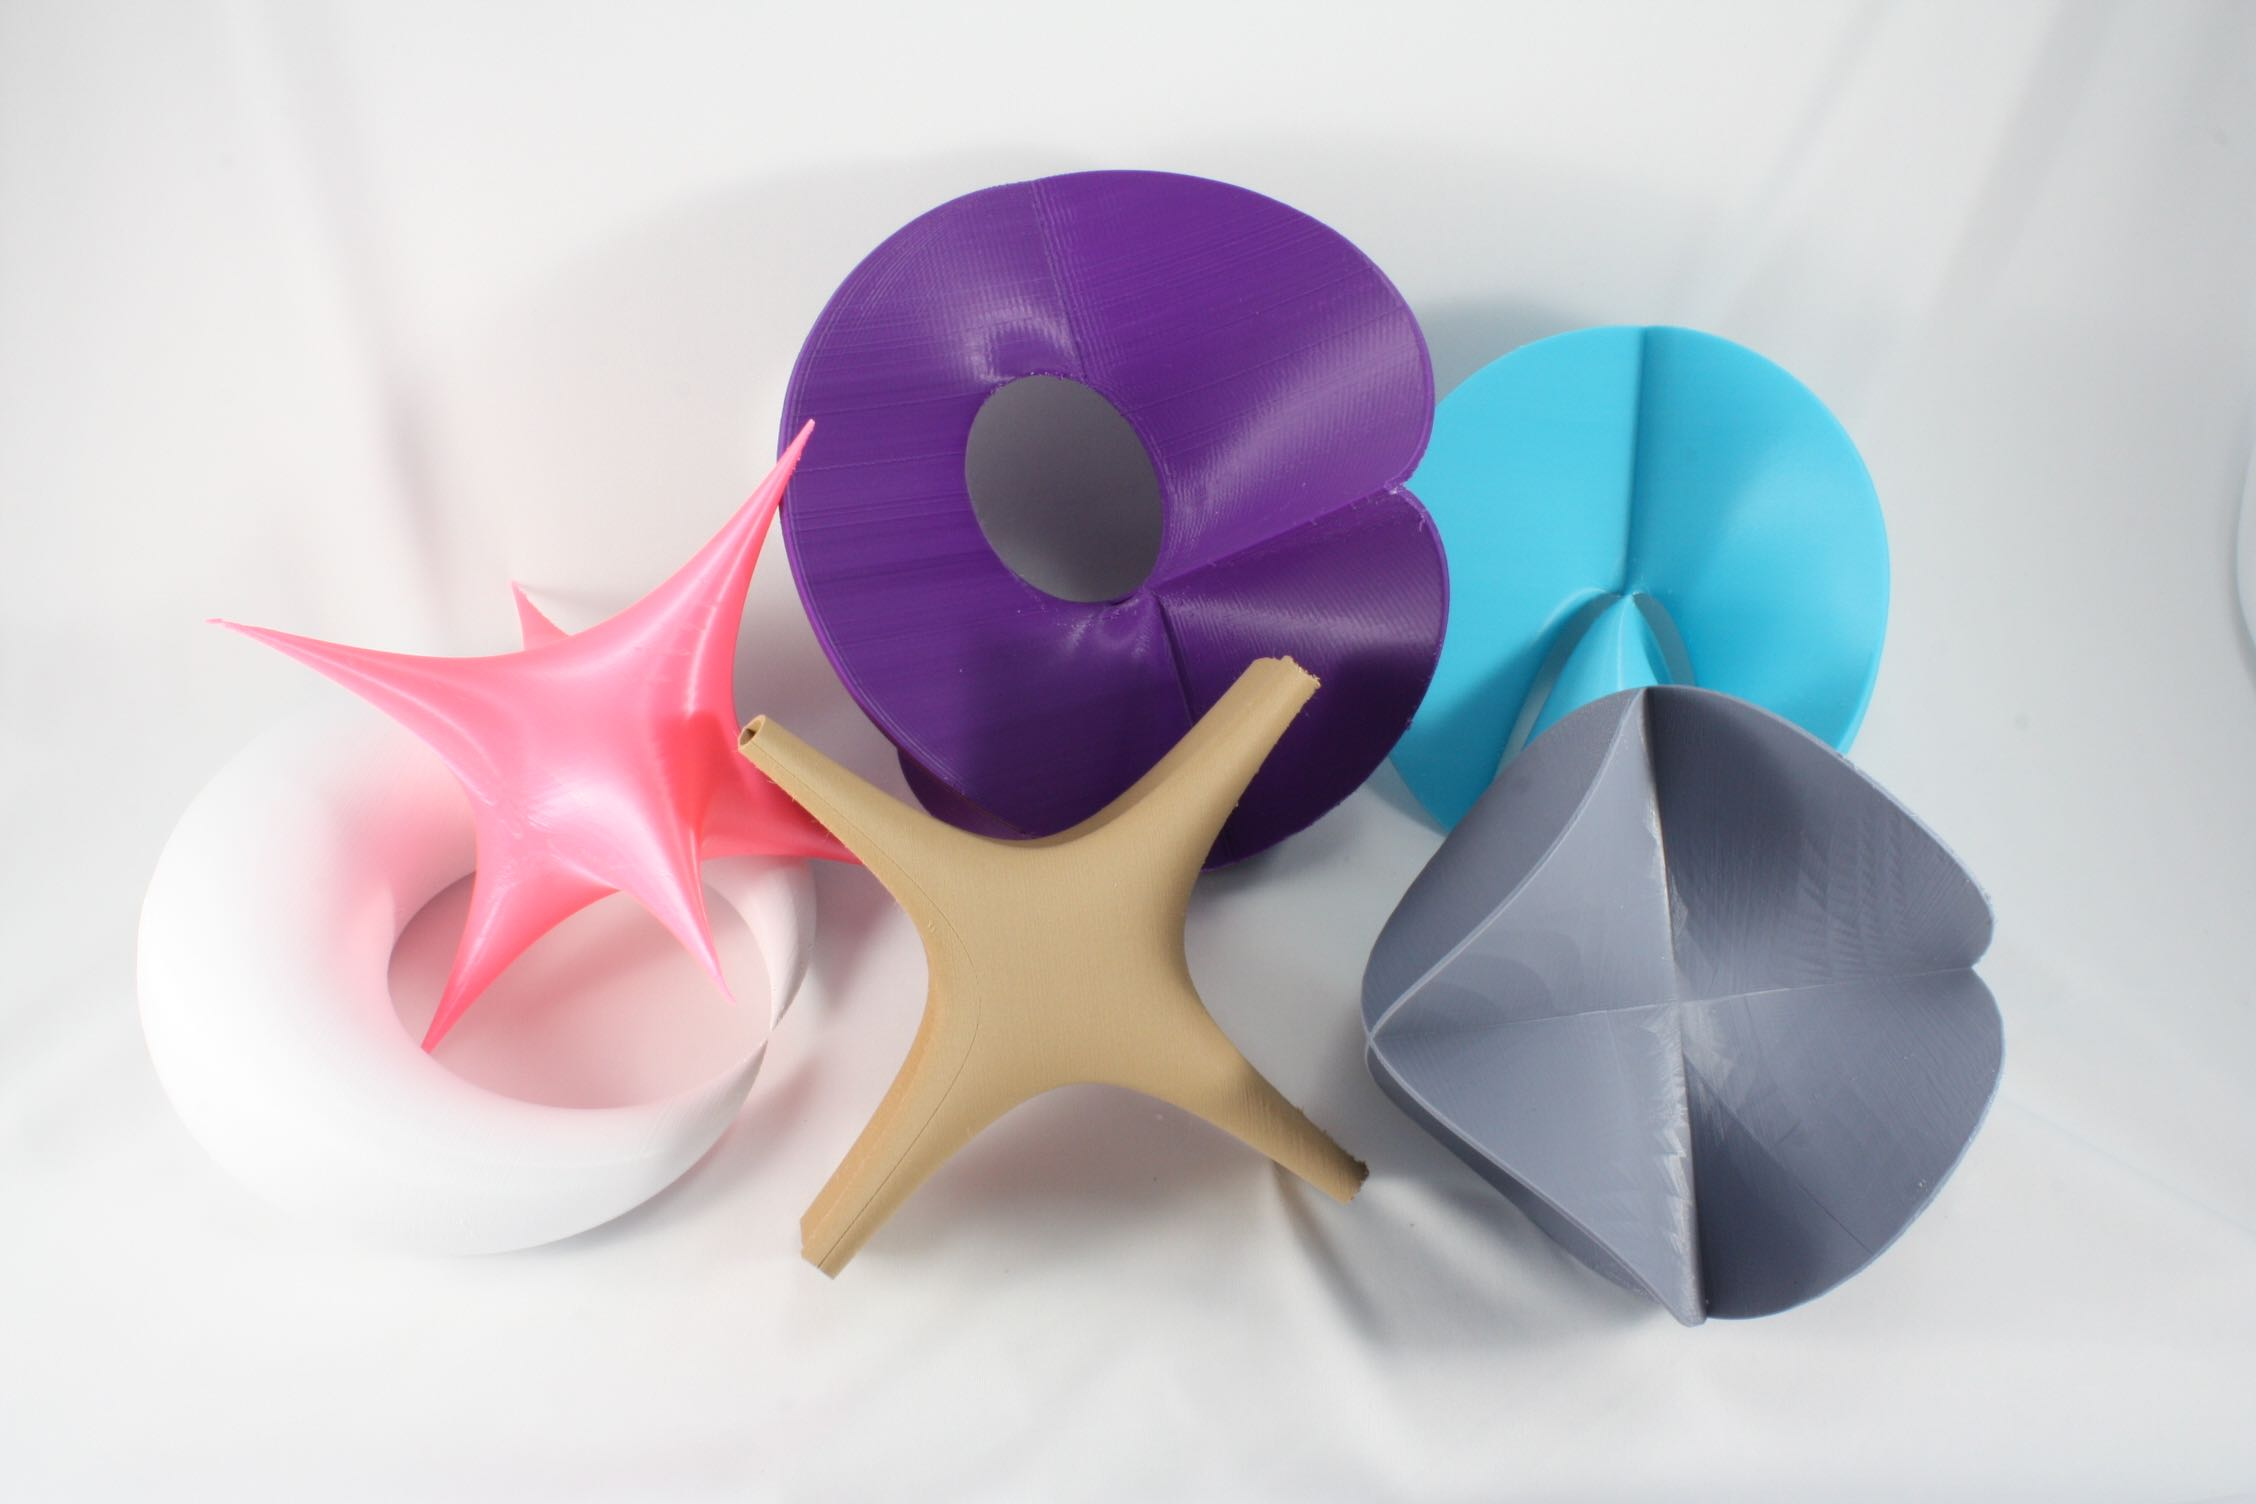
\includegraphics[width=\paperwidth]{diagrams/medley_croi_sol_tob_hel_ste_him.jpg}}%
\fframe{Thank you!}{


}











\end{document}


